\section{Evidence for Dark Matter}

Dark matter is one of the most mysterious problems cosmologists are faced with today. There is an overwhelming amount of observational evidence for the existence of this elusive substance. One such observation is found looking at galactic rotation curves. Classical mechanics tells us that the expected rotational velocity is defended by:

\begin{equation}
	V(r) \approx \sqrt{\frac{GM(r)}{r}}
\end{equation}

\noindent
giving the assumption that the velocity should drop off as $\frac{1}{r^{1/2}}$. As shown in figure 1, it can be seen that this is not the case. The rotational velocity of the stars remain constant as the distance from the center of the galaxy increases indicating that the mass varies as a function of $r$ as we move outside the visible edges of the galaxy.\cite{phipps_ionization_2016}

\begin{figure}[h]
	\centering
	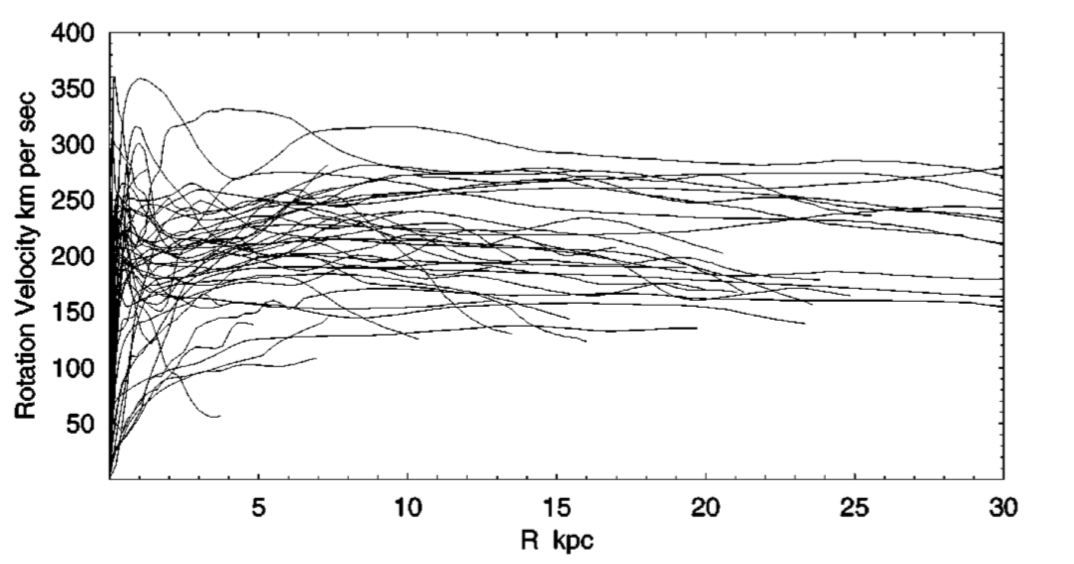
\includegraphics[scale=.7]{gal_vel}
	\caption{Galactic Velocity Distribution.\cite{phipps_ionization_2016}}
\end{figure}

\newpage
\section{Direct Detection}
Weakly Interaction Massive Particles (WIMPS) are a favorite candidate for particle dark matter. WIMPS may elastically scatter off nuclei with enough energy to be detected by current laboratory detectors. Measurements of the nuclear-recoil energy spectrum by these experiments can constrain the properties of WIMP dark matter as measurements below $1keVNr$ are required.\cite{agnese_cdmslite:_2014} Measuring a nuclear recoil at low energies does come with its difficulties. The measurements are constrained by the ability to subtract a background signal and the amount of exposure the detector gets as the expected WIMP-nucleon cross-section is only a few events per year. \cite{sorensen_atomic_2015} The sensitivity is also limited by the ability to distinguish between electron recoil and nuclear recoil events. \textbf{this needs reworking / more info.}


\section{Motivation and Preparation}

With the parameter space for WIMP dark matter candidates being pushed to lower energies, it has become important to accurately determine the deposited energy within the detector and the amount of charge liberated in each event. The fraction of charge liberated in an event is called the ionization yield. Specifically this fraction of charge is liberated in the form of electron-hole pairs. To calculate the variance in the ionization yield one needs to take into account a few phenomenon. Not all of the energy in a scattering event goes into creating electron hole pairs. There is a coupling mechanism to where some of the energy is deposited into the phonon system and the lower the particle energy, the more this factor plays a role.\cite{Transport} Variation in the amount of electron-hole pairs created from the energy deposited into the electronic system is also important, as a multiple events with the same energy don't always create the same amount of electron hole pairs. \par
\noindent
To date, these phenomenon have been accounted for, (see equation 3.1) but when comparing the current model to experimental data there is a significant difference in the spread of the data.\cite{Kennedy} There are a few reasons that this might be. One, the model that is used to find the nuclear recoil energies, the Lindhard model, has an energy dependent calculation that is not included in the variance calculation.\cite{Lindhard_3} Two, similar to electron recoils, there exists a nuclear "fano factor" that is also not included. The question is then this: Does including a nuclear recoil fano factor explain the difference in variance between the model and the data? If so, is there a energy dependent functional form to this fano factor? \par
\noindent
The Masters of Integrated Sciences program has prepared me for researching the content detailed in this research proposal. With my emphasis in mathematics, i have taken data analysis and statistical analysis. Theses courses will allow me to competently explain and understand the information necessary to determine the nuclear fano factor, as it will involve statistical modeling and error analysis. For my second emphasis, physics, i am taking graduate quantum mechanics. The combination of quantum and my class in numerical partial differential equations, I am confident that I can understand the physics necessary to look beyond the computational aspect of this project. 


 





